\section{twinX}

Una vez hemos analizado el material ya existente y desde el que partiremos para la construcción de twinX, vamos a ponernos manos a la obra con su desarrollo. Si bien es cierto que no se parte desde cero en cuanto a requisitos, sí que se va a reconstruir la herramienta desde cero, para poder aportar un gran significado a todos los módulos que vayan a formar parte de twinX y así podamos cohesionarlos de una mejor manera.

\subsection{Desarrollo de twinX}

Vamos a comenzar estableciendo las ideas principales del proyecto, reafirmando el propósito y viéndolo desde otras perspectivas que, aunque parecen obvias, no siempre se tienen en cuenta. Ello nos permitirá asentar las bases del producto software final y dotarlo de calidad.

\subsubsection{Diseño centrado en el usuario}

Esta disciplina, conocida también como \textit{User-Centered Design} o UCD, destaca por basar las fases del proceso de diseño estableciendo un enfoque constante en aprender del sujeto que utilizará el producto final. Es decir, para la consecución de los objetivos, es necesario tener una retroalimentación constante por parte del usuario final, que será quien vaya orientando nuestros avances según sea su interacción con lo que vayamos desarrollando.

El proceso dispone de unas fases a seguir, como son:
\begin{itemize}
	\item \textbf{Especificación del contexto de uso:} quiénes usarán el producto, para qué y bajo qué condiciones lo harán.
	\item \textbf{Especificación de requisitos:} identificar los objetivos que tienen que cumplirse para dejar a los usuarios satisfechos.
	\item \textbf{Crear soluciones de diseño:} en distintas etapas, desde un concepto poco definido hasta un diseño completo.
	\item \textbf{Evaluación de los diseños:} a través de las pruebas con los usuarios, de forma ideal.
\end{itemize}

\paragraph{Pautas de Accesibilidad}
\leavevmode\\[\baselineskip]

El no atender a causas de accesibilidad sería no aplicar correctamente, de alguna forma, el tipo de diseño escogido para el desarrollo del producto. Cuando se hacen pruebas, el objetivo no es otro que adaptar el producto para que pueda ser bien utilizado por el mayor número de usuarios posible y de la forma satisfactoria para ellos. Es por ello por lo que tenemos que abrir el abanico y contemplar que pueden ser numerosos los usuarios que necesiten adaptaciones para interaccionar correctamente con el contenido web.

Para ello, se propone la utilización de los recursos especificados en \textit{Web Content Accessibility Guidelines} (WCAG) \citep{wcag}. Con ello, podemos hacer que la experiencia en el sitio web pueda ser mínimamente satisfactoria para todo usuario que necesite hacer uso de la misma. Para ello, se deberán emplear una serie de técnicas, especificadas en su web, para que twinX sea adaptable. Entre ellas, destacamos la posibilidad de interacción con el teclado, un texto descriptivo para las posibles imágenes que se puedan incluir, regular el contraste, etc. Con este proyecto, la intención es alcanzar el nivel AA (segundo más exigente), para que la gran mayoría de personas con necesidades especiales puedan usar la plataforma sin problema alguno.

\paragraph{Encuesta SUS}
\leavevmode\\[\baselineskip]

[Pendiente de revisión]

\subsubsection{\textit{Design Thinking}, DT}

El « Pensamiento de Diseño » o \textit{Design thinking} es una técnica de desarrollo que se centra en el usuario, pudiendo detectar y reaccionar ante cambios repentinos en el entorno de los usuarios y sus comportamientos. El objetivo está, mayormente, en abordar problemas con una pobre definición o que no se conocen a fondo para situar al usuario en el centro de todo y poder así enfocar el problema desde otras perspectivas, de manera que se pueda poner la atención en aquello que resulte de mayor importancia para los usuarios.

\paragraph{Las fases del DT}
\leavevmode\\[\baselineskip]

El proceso tiene unas fases no necesariamente secuenciales, de modo que puedan adaptarse lo mejor posible al proyecto, teniendo incluso la posibilidad de ejecutarse al mismo tiempo.

\begin{itemize}
	\item \textbf{Empatizar}, tratar de adoptar un conocimiento lo más empático posible del problema que se pretende resolver. Este es un elemento esencial, pues posibilita a los desarrolladores a descartar sus propias primeras conclusiones --erróneas a menudo-- y a entrar en materia con la realidad del cliente y sus necesidades.
	
	\item \textbf{Definir} las necesidades de los usuarios y sus problemas. Es la fase donde se reúnen y ordenan los elementos obtenidos como resultado de la fase anterior. A partir de entonces, se sintetizan para definir los problemas esenciales que se identifican, los cuales dan pie a la creación de \textit{personas}; esto es, la construcción de perfiles humanos en los cuales centrar el desarrollo.
	
	\item \textbf{Idear} y hacer frente a lo que se da por hecho, creando formas alternativas de ver y tratar el problema con soluciones innovadoras, a partir de lo estudiado en las dos fases anteriores.
	
	\item \textbf{Prototipado} de las soluciones pensadas, una fase experimental cuyo objetivo es el de encontrar la mejor solución para cada uno de los problemas encontrados. Los desarrolladores han de producir una versión de bajo coste del producto para investigar cuál es el resultado de haber llevado las ideas a la práctica.
	
	\item \textbf{Pruebas} con lo obtenido, para analizar si realmente se ha llegado a un buen resultado o, si por el contrario, se ha de retroceder a otra fase para redefinir uno o más problemas.
	
\end{itemize}

Como hemos indicado, las fases no siempre siguen el mismo orden. Hay veces que se toman decisiones como la de saltar de la primera fase de empatía a la penúltima de prototipado, probablemente para aclarar las ideas y poder hacer una mejor definición, a través de la muestra de material al cliente que pueda animarlo a dar una mayor retroalimentación. Del mismo modo, si el prototipado no ha ido bien, se puede volver a la tercera y anterior fase, la de construcción de ideas. Incluso podría darse el caso que haciendo pruebas, los desarrolladores nos demos cuenta de que no se ha llevado a cabo una buena ejecución del proceso y sea preciso volver a la segunda etapa de definición de los problemas. Siempre es mejor ir hacia atrás en lugar de comenzar la casa por el tejado, así que toda maniobra que sea apropiada para una mejor construcción del producto y que lo dote de calidad siempre es bienvenida.


\paragraph{Herramientas del DT}
\label{herramientasDT}
\leavevmode\\[\baselineskip]

Hay una serie de actividades o técnicas que nos pueden resultar útiles para llevar a cabo el trabajo de desarrollo con eficacia y que suelen tener éxito. Destacamos las siguientes:

\begin{itemize}
	\item \textbf{Creación de personas:} perfiles ficticios de los distintos usuarios que utilizarán el producto software. Creadas en la fase de definición, no solo se especifica el propósito específico de interacción con el producto a mejorar o la necesidad por que exista el software que se quiere desarrollar. Describimos el contexto del personaje, sus inquietudes y, en definitiva, lo que hay detrás de esa persona en más ámbitos que puedan ayudar a comprender por qué es necesario que se tengan en cuenta ciertas cosas a la hora del desarrollo.
	
	\item \textbf{\textit{Brainstorming}:} también conocida como nube de ideas que radican alrededor de un concepto central. Se trata de escribir conceptos que vengan a la cabeza de los intervinientes en la creación del esquema, sin importar los análisis o el futuro que puedan tener en el proceso. Cualquier cosa que tenga que ver con lo que se está tratando es válida, pues lo que aparentemente resulta absurdo podría en muchos casos resolver parcialmente el problema o ayudar a enfocarlo. Así, cuantas más propuestas, mejor se lleva a cabo este proceso, que tiene lugar en la fase de ideación.
	
	\item \textbf{Prototipado en papel:} la creación de prototipos (en la cuarta fase de prototipado) con un material del que todos disponemos es extremadamente sencilla a la par que útil. Cuando las cosas se plasman en un folio, podemos apreciar matices que no nos venían a la cabeza cuando la idea era tan solo un concepto. Si bien es cierto que depende de las dotes artísticas de la persona que dibuja el prototipo, el hacerlo con papel y lápiz ayuda a volcar la concentración de una manera diferente a como se hace cuando se programa o se diseña con herramientas informáticas.
	
	\item \textbf{Mapas de experiencia de usuario:} también conocidos como \textit{Customer Journey Maps}, sirven para representar la experiencia de un usuario a lo largo del tiempo. En ellos plasmamos la forma en que un diseño cubre o no las necesidades de un usuario utilizando un producto o servicio. Es justo por eso por lo que estos mapas han de ser lo más descriptivos posibles, representando con gran detalle las acciones y subtareas que tiene que desempeñar un usuario al usar el sistema.
	
\end{itemize}

\subsubsection{Aplicación de las metodologías}

En relación con las fases del DT, podemos diferenciar a través de las cuales ya hemos ido pasando. El comienzo del proyecto vino acompañado de una serie de reuniones que se incluyen en los anexos. En este contexto, la fase de \textbf{empatización} se correspondería con las dos primeras reuniones, donde se establecieron un primer contacto y las bases del proyecto, atendiendo al testimonio de los usuarios reales de TWINS, lo que actualmente se está usando para resolver los problemas a los que se tienen que enfrentar en la ORI-FyL. Es más, en la reunión segunda (\ref{reunion2}) se habló de algunas características ideales y que está costando implementar en el actual escenario, lo que podríamos englobar dentro de la \textbf{ideación}. Por último, ya en la tercera reunión, se tiene la \textbf{definición} de todos los conceptos necesarios para comprender el funcionamiento de TWINS y de la oficina en general. No obstante, a lo largo de esta sección, vamos a continuar esta fase con la definición de más elementos necesarios para llevar a cabo el desarrollo de twinX.

Con esas tres fases cubiertas, se puede dar comienzo a las otras dos: la de \textbf{prototipado} y \textbf{pruebas}, que serán desarrolladas de forma más extensa en las secciones ~\ref{bocetos} y ~\ref{pruebas}. %PENDIENTE: comprobar referencias, ya que han sido puestas antes de tiempo y añadir posibles futuras reuniones y sesiones de pruebas.

\subsection{Personas ficticias}

Tal y como hemos comentado en la sección \ref{herramientasDT}, una de las herramientas que nos permiten definir el alcance y las necesidades de la aplicación es la creación de perfiles de personas ficticias, candidatos a utilizar twinX en un futuro. De esta forma, tanto por la parte del desarrollo como por la del interesado en el producto final, pueden no solo hacerse una mejor idea de los objetivos del mismo, sino también justificar su creación.

Vamos a tratar de crear tres personalidades lo más variopintas posibles en aras de hacer esta herramienta lo más útil posible, de modo que podamos abarcar por completo el entorno de influencia del problema. (Herramienta: \citep{xtensio})

\begin{figure}
	\centering
	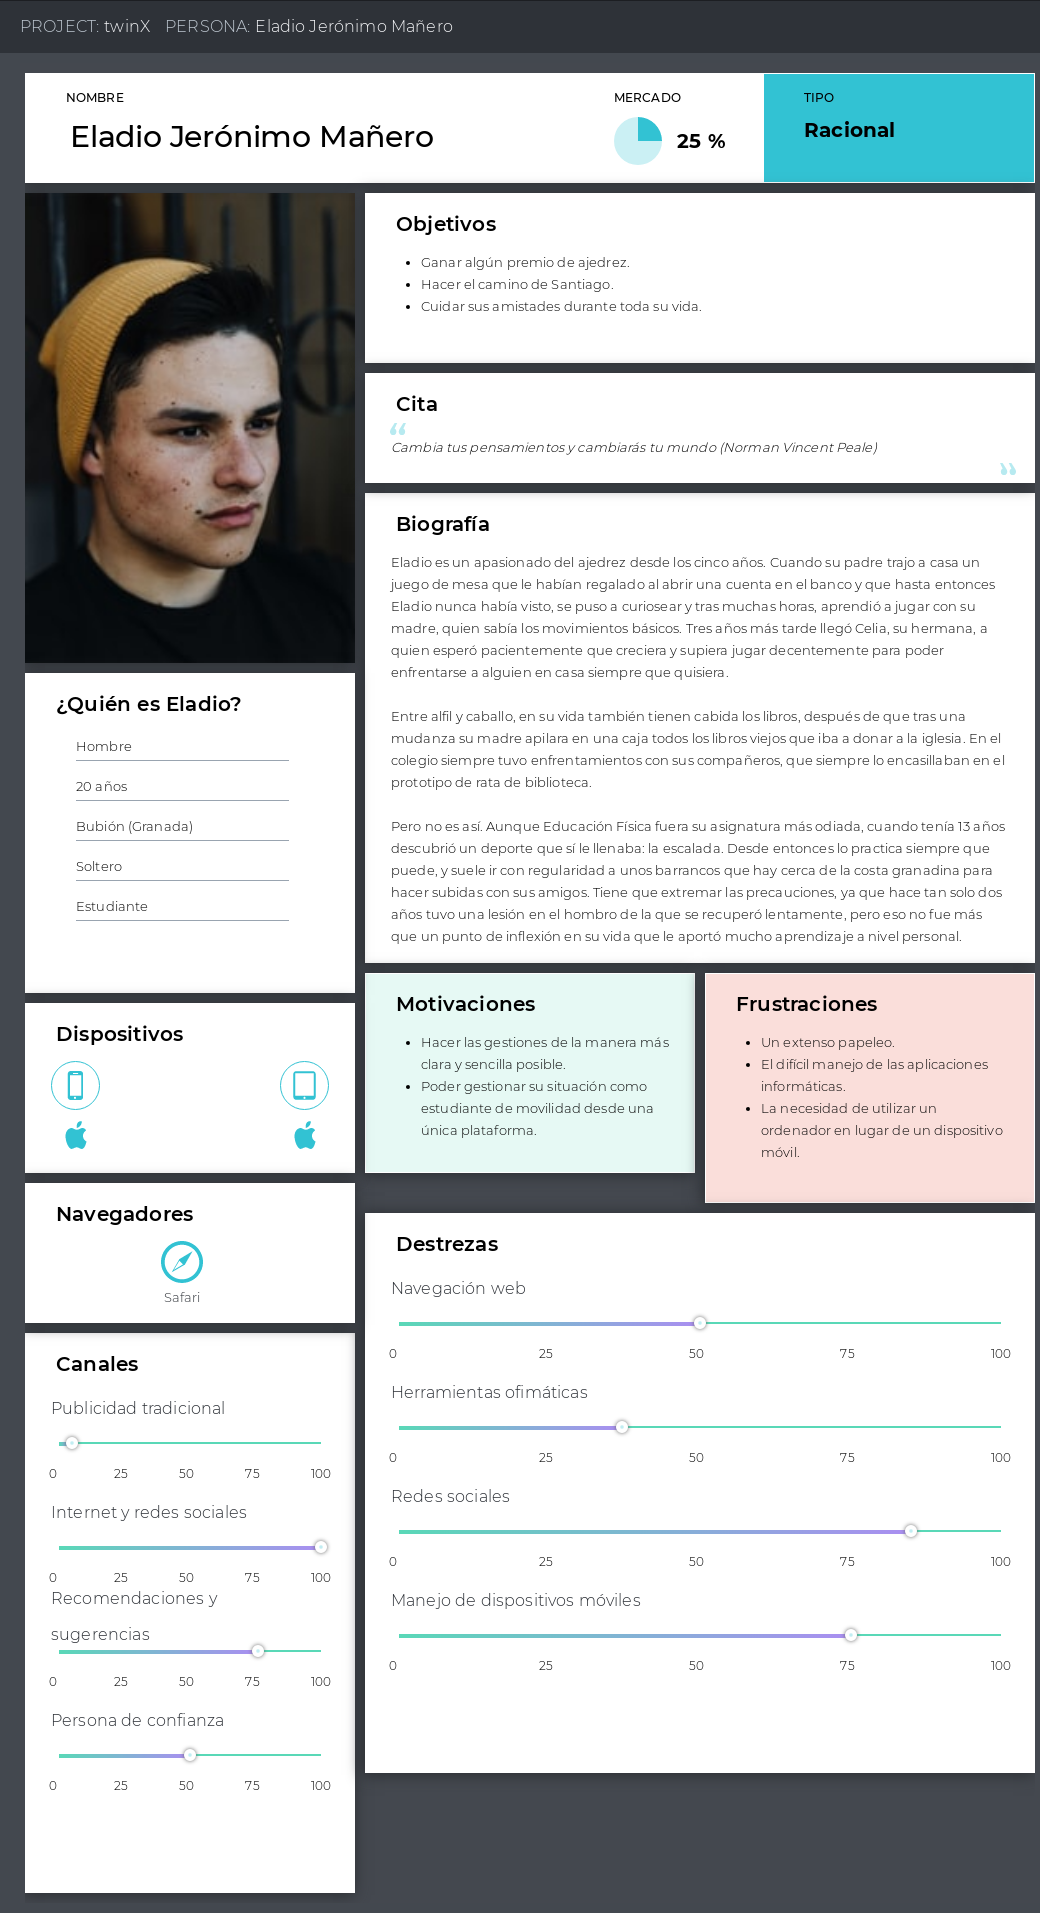
\includegraphics[width=\textwidth]{img/Personas/Eladio}
	\caption[Persona \#1]{Persona \#1: Eladio}
	\label{fig:persona1}
\end{figure}

% Dos personas más, pendiente de revisión la primera.

\subsection{Entrevistas}
[Pendiente de revisión]

\subsection{Malla receptora de la información}




%%%%%% SECCIÓN 3.5
%\subsection{Descripción de la propuesta}
%
%Para desarrollar twinX primero se ha de elegir una metodología. En este caso, dado que este proyecto es tan sólo un comienzo para lo que sería el producto final y que tiene unos requisitos poco cerrados, escogeremos una metodología de desarrollo ágil.
%
%Este tipo de metodologías se basan en la adaptación a medios con necesidades cambiantes, con un desarrollo muy de cerca con el cliente, quien está presente junto con el equipo de desarrollo en las numerosas reuniones que se hacen a lo largo de la vida del proyecto. En este caso, el equipo de desarrollo es ajustado, pero no por ello dejaremos de lado la necesaria intervención de dos personas que hacen el papel de clientes y que son:
%
%\begin{itemize}
%	\item María Consuelo Pérez Ocaña (Coordinadora de Internacionalización en la la Facultad de Filosofía y Letras)
%	\item Miguel Ángel Sanz Sáez (personal de secretaría y creador de TWINS)
%\end{itemize}